\documentclass{standalone}
\usepackage{tikz}
\begin{document}
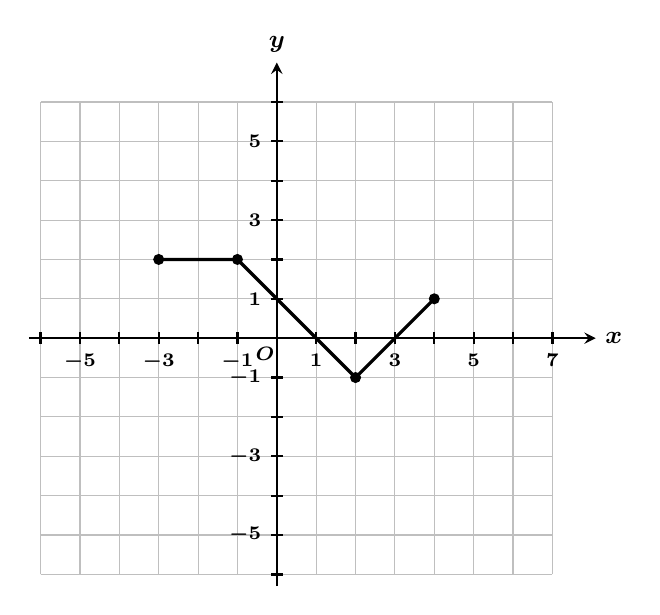
\begin{tikzpicture}[color=black, >=stealth, scale=0.5]
  % Grid: x from -6 to 7, y from -6 to 6
  \draw[gray!50, thin] (-6,-6) grid (7,6);
  % Axes: plain ends on the negative side, arrows on the positive side
  \draw[->, thick] (-6.3,0) -- (8.1,0);
  \draw[->, thick] (0,-6.3) -- (0,7);
  \node[font=\small\boldmath, anchor=west] at (8.1,0) {$x$};
  \node[font=\small\boldmath, anchor=south] at (0,7) {$y$};
  \node[font=\scriptsize\boldmath] at (-0.3,-0.4) {$O$};
  % Tick marks at every integer
  \foreach \t in {-6,...,7}
    \draw[thick] (\t,0.15) -- (\t,-0.15);
  \foreach \t in {-6,...,6}
    \draw[thick] (0.15,\t) -- (-0.15,\t);
  % Tick labels at odd values
  \foreach \t in {-5,-3,-1,1,3,5,7}
    \node[font=\scriptsize\boldmath, anchor=north] at (\t,-0.15) {$\t$};
  \foreach \t in {-5,-3,-1,1,3,5}
    \node[font=\scriptsize\boldmath, anchor=east] at (-0.15,\t) {$\t$};
  % Piecewise-linear graph with filled endpoints and corners
  \draw[line width=1.2pt] (-3,2) -- (-1,2) -- (2,-1) -- (4,1);
  \fill[black] (-3,2) circle (4pt);
  \fill[black] (-1,2) circle (4pt);
  \fill[black] (2,-1) circle (4pt);
  \fill[black] (4,1) circle (4pt);
\end{tikzpicture}
\end{document}
